\chapter{An Unsupervised Learning Paradigm for MIMO User Scheduling} \label{usch:chap}

%In this chapter we propose and design a novel, simple, and practical unsupervised learning approach to MAC user scheduling based on uplink CSI knowledge.
%Unlike supervised learning, which would require a large number of labeled training channels, our unsupervised MAC user scheduling can directly operate on knowledge of user uplink channel state information (CSI) to mitigate multiple access interference (MAI) among users and to achieve high MAC capacity. 
%Our novel methodology starts by classifying users into high similarity groups through learning based on a novel metric of projected CSI similarity. 
%We then develop a simple MAC protocol by only scheduling users from user groups with high inter-cluster distance for joint access to mitigate multiple access interference (MAI). 
%We provide comprehensive performance evaluations of the proposed  MAC scheduling protocol in terms of spectral  efficiency, bit-error-ratio, user fairness, and robustness.


In this chapter, we propose an effective and scalable user scheduling based on unsupervised learning. 
Given channel state information (CSI) of users, we first apply unsupervised learning to identify mobile users with highly similar CSI. 
We develop a new scheduling principle to enhance spatial diversity by dispersing users of high CSI similarity into different MIMO access groups. 
We formulate a user clustering problem over Grassmannian manifold to identify users that can pose strong co-channel interference. 
We consider downlink MIMO and uplink MIMO, with or without power control for simple implementation. 
Our new scheduling approach is generalizable to a variety of different simple and scalable unsupervised learning tools and different diversity optimization criteria. 
Numerical tests demonstrate the substantial gain in terms of spectrum efficiency and interference suppression at modest computation complexity. 
\crfootnote{Part of this chapter has been previously submitted to \textit{IEEE Transactions on Wireless Communications} and is currently under review.}


\section{The Scheduling Problem}\label{usch:sec:systemmodel}

% from II.E: 
Previous works on resource-sharing MIMO systems have studied optimal decoder (MAC) and precoder (BC) designs that achieve channel capacity for a given resource-sharing group, such as the MMSE-SIC receiver \cite{Tse05} for MAC or dirty-paper precoding \cite{Costa1983} with MMSE filters for BC. 
However, these designs were proposed with the premise that users have already been scheduled in MIMO user groups.
To benefit from these exciting works in the literature, we investigate the scheduling problem that is a foundation step to MIMO precoding and rate maximization. 

In the following, we adopt the system model developed in Section~\ref{system:sec:usch}. We assume similar data rate requirements for all users, and thus we use spectrum efficiency as performance metric.  Hence, we first obtain the spectrum efficiency in terms of co-channel interference and user rates. Note that because the system model assumes single-carrier systems, we use normalized bandwidth.

\subsection{Co-Channel Interference and Sum-Rate}
The interference that user $u\in\mathcal{S}_g$ experiences is measured by their signal-to-interference-and-noise ratio or SINR. In the case of MAC, the SINR of user $u$ is 
\begin{align}
	\SINR_u^{\MAC} = \frac{p_u|\bm{W}_g\herm\bm{h}_u|^2}{\sigma^2+\sum_{i\in\mathcal{S}_{g},i\neq u}p_i|\bm{W}_g\herm\bm{h}_i|^2}.
	\label{usch:eqn:sinr_mac}
\end{align}

Among several receiver designs, without loss of generality we adopt the MMSE receivers \cite{Tse05} for their straightforward implementation and to fully leverage spatial diversity. In the $g$-th group, the MMSE design defines the column of the $g$-th decoder matrix $\bm{W}_g$ corresponding to user $u\in\mathcal{S}_g$ as 
\begin{align}
	\bm{W}_{g}=\bigg(\sigma^2\bm{I}_M+\sum_{i\in\mathcal{S}_g,i\neq u} p_i\bm{h}_i\bm{h}_i\herm\bigg)^{-1}\bm{h}_u,
\end{align}
with a resulting SINR of
\begin{align}
	\SINR_u^{\MAC} = p_u\bm{h}_u\herm\bigg(\sigma^2\bm{I}_M+\sum_{i\in\mathcal{S}_g,i\neq u} p_i\bm{h}_i\bm{h}_i\herm\bigg)^{-1}\bm{h}_u.
	\label{usch:eqn:sinr_mac_mrc}
\end{align}

For BC, the SINR of user $u$ corresponds to 
\begin{equation}
	\SINR_u^{\BC} = \frac{p_u|\bm{h}_u\T\bm{z}_u|^2}{\sigma^2+\sum_{i\in\mathcal{S}_{g},i\neq u}p_i|\bm{h}_u\T\bm{z}_i|^2},
	% \SINR_u^{\BC} = \frac{p_u|\bm{h}_u\herm\bm{z}_u|^2}{\sigma^2+\sum_{i\in\mathcal{S}_{g(n)},i\neq n}p_i|\bm{h}_u\herm\bm{z}_i|^2}.
	\label{usch:eqn:sinr_bc}
\end{equation}
and, without loss of generality and for the sake of simplicity, we use the MRT precoders \cite{Lo1999mrt}
\begin{equation}
	\bm{z}_u=\frac{\overline{\bm{h}_u}}{\|\bm{h}_u\|}\,,\,\,\forall u\in\{1,\ldots,N\},
\end{equation}
which yield a resulting SINR for user $u$ of
\begin{equation}
	\SINR_u^{\BC} = \frac{p_u\|\bm{h}_u\|^2}{\sigma^2+\sum_{i\in\mathcal{S}_{g},i\neq u}p_i|\bm{h}_u\T\overline{\bm{h}_i}|^2/\|\bm{h}_i\|^2}.\label{usch:eqn:sinr_bc_mrt}
	% \SINR_u^{\BC} = \frac{p_u\|\bm{h}_u\|^2}{\sigma^2+\sum_{i\in\mathcal{S}_{g(n)},i\neq n}p_i|\bm{h}_i\herm\bm{h}_u|^2/\|\bm{h}_u\|^2},
\end{equation}

The normalized sum-rate of the $g$-th group is given by 
\begin{align}
	R_g&=\sum_{u\in\mathcal{S}_g}\log_2\big(1+\SINR_u\big),\label{usch:eqn:sum_rate}
\end{align}
with $R_g^{\MAC}$ and $R_g^{\BC}$ denoting the sum-rates for uplink and downlink, respectively, using the corresponding expressions for SINR. 

% Additionally, it is well known that for a given transmission power distribution $\bm{P}$, the achievable sum-rate of a scheduled group $g$ is obtained with linear MMSE filters \cite{Tse05} in both uplink and downlink, and is given by
% \begin{equation}
	% 	\hat{R}_g={\log _2}\det\left( \bm{I}_M +\sigma^{-2} \bm{H}\bm{\Pi}_g\bm{P}\bm{\Pi}_g\bm{H}\herm \right).\label{usch:eqn:max_rate}
	% \end{equation}
% whereas the MMSE receiver yields a user SINR \cite{Tse05}
% \begin{align}
	%     \SINR_u^{\MAC}&=p_u\bm{h}_u\herm\Big(\sigma^2\bm{I}_M+\sum_{i\in\mathcal{S}_{g},i\neq n}p_i\bm{h}_i\bm{h}_i\herm\Big)^{-1}\bm{h}_u.
	%     % &=\frac{1}{\Big(\big(\bm{I}_{|\mathcal{S}_{g}|}+\sigma^{-2}\bm{H}_{g}\herm\bm{P}_{g}\bm{H}_{g}\big)^{-1}\Big)_{\underline{n},\underline{n}}}-1,
	%     % \SINR_u^{\MAC}&=p_u\bm{h}_u\herm\Big(\sigma^2\bm{I}_M+\sum_{i\in\mathcal{S}_{g(n)},i\neq n}\bm{h}_i\bm{h}_i\herm\Big)^{-1}\bm{h}_u\nonumber\\
	%     % &=\frac{1}{\Big(\big(\bm{I}_{|\mathcal{S}_{g(n)}|}+\sigma^{-2}\bm{H}_{g(n)}\herm\bm{P}_{g(n)}\bm{H}_{g(n)}\big)^{-1}\Big)_{\underline{n},\underline{n}}}-1,
	%     \label{usch:eqn:sinr_mac_mmse}
	% \end{align}

% Now, the capacity of group $g$ corresponds to the maximum achievable rate possible with optimal power allocation, subject to a limited sum power for the group $P_{\mathrm{max}}$, i.e.
% \begin{equation}
	% 	C_g=\max_{\bm{P}\,:\,\Tr(\bm{\Pi}_g\bm{P}\bm{\Pi}_g)\leq P_{\mathrm{max}}} \hat{R}_g.\label{usch:eqn:capacity}
	% \end{equation}



% \textcolor{magenta}{where ${\bm{\Sigma}_g} ={\bm{x}}_g{\bm{x}_g}\herm$ is a $M\times M$ symmetric matrix, which denotes the users that we select to share $b$-th RB.}

% \textcolor{red}{Carlos: Either discuss power allocation difficulty here, and avoid that discussion later, or add power in the scheduling problem and then dismiss it. I'm inclined for option 1, as it is more straightforward.}

\subsection{Problem Formulation}
Ideally, we aim to optimize the design of the indicator 
% matrices $\bm{\Pi}$ and power allocation $\bm{P}$ 
variables $\pi_{g,u}$ and user power allocation $p_u$
to maximize the efficiency of resource usage in terms of sum rate, that is, maximizing the sum-rate of each RSG and minimizing the number of groups simultaneously. 
A mathematical formulation of this approach, valid for either MAC or BC scheduling, is %{C_{\rm{sum}}}\left( \Pi  \right)
\begin{subequations}\label{usch:eqn:sumrate_optimization}
	\begin{align}
		\mathcal{P}^{}:\max_{G,\;\pi_{g,u},\;\,p_u} &\quad\frac{1}{G}\sum\nolimits_{g =1}^{G} R_g^{}\label{usch:eqn:optimization_obj}\\
		\text{s.t.}  
		% 		&\quad\bm{1}_N\T\bm{\Pi}_{g}\bm{1}_N\leq M,\,\, \forall g\,\in\{1,\ldots,G\},\label{usch:eqn:optimization_userConstraint}\\
		&\quad\sum\nolimits_{u=1}^N\pi_{g,u}\leq M,\,\, \forall g\,,\label{usch:eqn:optimization_userConstraint}\\
		%  		&\quad\diag(\bm{\Pi}_g)\in\{0,1\}^N,\,\, \forall g\,\in\{1,\ldots,G\}%\,\,.\label{usch:eqn:optimization_binaryExclusivity}
		%  		,\label{usch:eqn:optimization_binaryExclusivity}\\
		&\quad\pi_{g,u}\in\{0,1\},\,\, \forall g\,,\forall u\,
		,\label{usch:eqn:optimization_binaryExclusivity}\\
		% 		&\quad\Tr(\bm{\Pi}_g\bm{P}\bm{\Pi}_g)\leq p_{\mathrm{BS}}^{\mathrm{max}},\,\, \forall g\text{ (BC)},\label{usch:eqn:optimization_powerAllocation_bc}\\
		&\quad \sum\nolimits_{n=1}^N p_u\pi_{g,u}\leq p_{\mathrm{BS}}^{\mathrm{max}},\,\, \forall g\text{ (BC)},\label{usch:eqn:optimization_powerAllocation_bc}\\
		&\quad0\leq p_u\leq p_{\mathrm{UE}}^{\mathrm{max}},\,\, \forall n\text{ (MAC)}.\label{usch:eqn:optimization_powerAllocation_mac}
	\end{align}
\end{subequations}
% point back to exclusivity and binary variables

In Problem ${\cal P}$, constraint (\ref{usch:eqn:optimization_userConstraint}) limits the number of MAC/BC users up to the number of BS antennas $M$ without requiring further non-orthogonal multiple access. By design, each user belongs to one group only (\ref{usch:eqn:optimization_binaryExclusivity}). Additionally, in practical BC systems the BS transmission power is limited by $p_{\mathrm{BS}}^{\mathrm{max}}$ in every time slot and needs to be properly allocated (\ref{usch:eqn:optimization_powerAllocation_bc}), whereas in MAC each user has a maximum transmission power $p_{\mathrm{UE}}^{\mathrm{max}}$ (\ref{usch:eqn:optimization_powerAllocation_mac}).
In order to further mitigate CCI, additional constraints can be considered when more design parameters are available, such as 
resource availability, cooperation in BC, individual rate requirements, among other criteria.
% (\ref{usch:power}) enforces a peak user power constraint $P_{\max}$ and, depending on practical considerations, the individual power constraint of (\ref{usch:power}) may be replaced by a total sum power constraint of $0<\sum_{n=1}^N p_u\leq P_{\mathrm{sum}}$ or group power constraints $0<\sum_{n\in\mathcal{S}_g} p_u\leq P_{g,\mathrm{sum}}$ to mitigate sum inter-cell interference. 
Note that our formulation of problem ${\cal P}$ for maximizing spectrum efficiency can be modified as required to attain different objectives, and as such is without loss of generality. Other tractable performance metrics for MAC/BC user scheduling include the minimization of MSE \cite{Mo09, Lee76}, weighted MSE \cite{Sampath01}, maximization of SINR \cite{Scaglione99}, or minimization of BER \cite{Palomar05},
among others. 

Regardless of the selected objective, $\mathcal{P}$ is NP-hard and shares similar complexity as general nonlinear mixed integer programming. 
% \subsection{Problem Complexity}
To find the optimum MAC/BC user grouping $\pi_{g,u}^{\star}$, a direct exhaustive search method would need to evaluate all possible $\pi_{g,u}$ in terms of mean sum-rate (\ref{usch:eqn:optimization_obj}) to determine the optimum MAC/BC user grouping solution that achieves the 
best spectrum efficiency. However, the resulting search space is combinatorial even with a modest number of users and fixed $G$ and $p_u$, and as such requires very high computational load. 


% \textcolor{red}{NOT SURE what this paragraph is trying to say:  Similarly, optimizing power allocation, while enabling the improvement of total sum-rate, increases the dimension of the search space (increasing computational difficulty), and can also hinder fairness as users that enjoy larger channel gains could be benefited with larger power allocation whereas users with weaker CSI gains could be starved. }
% Therefore, a scalable solution imposes the use of simple transmit precoder and receive decoder designs, as proposed above for our BC and MAC system settings.

% \textcolor{blue}{Let suppose we perform $Q$ selections to obtain $Q$ user groups, and $m_q$ is the number of selected users in each selection. Recall that $N$ is the maximum number of users at each group. Therefore, the total possible combinations with exhaustive search are}
% \begin{align}
	% T&=\sum\limits_{{m_1} = 0}^{\min \left( {{S_{\max }}, M} \right)} {\binom{M_1}{m_1}}\sum\limits_{{m_2} = 0}^{\min \left( {{S_{\max }}, M - {m_1}} \right)} {\binom{M_2}{m_2}} \nonumber\\
	% &\times\sum\limits_{{m_3} = 0}^{\min \left( {{S_{\max }},M - {m_1} - {m_2}} \right)} {\binom{M_3}{m_3}}\cdots\nonumber\\
	% &\times\sum\limits_{{m_q} = 0}^{\min \left( {{S_{\max }}, M - \sum\nolimits_{j = 1}^{Q - 1} {{m_q}} } \right)} {\binom{M_Q}{m_Q}}.
	% \end{align}
% Such approach requires very high computation complexity. 
% For $M$ antennas, we may divide users
% into $G$ groups such that $\left\lceil {\frac{N}{M}} \right\rceil  \le G
% \le M$. By using \emph{Bell number} and \emph{Stirling numbers of the second kind}, 
% the exact number of ways of partitioning $N$ users into $G$ non-empty disjoint groups equals
% \begin{equation}\label{usch:bf}
	% 	T = {B_N} - \sum\nolimits_{G = 0}^{\left\lceil {\frac{N}{M}} \right\rceil }{S(N, G)},
	% \end{equation}
% where the Bell number ${B_N} = \sum\nolimits_{q = 0}^N S(N, q)$ is the number of ways of partitioning a set with $N$ elements into disjoint subsets and the Stirling numbers of the second kind $S(N, q)$ is the number of ways of partitioning $N$ users into $q$ non-empty and disjoint groups \cite{Riordan80}. By using a number triangle resembling Pascal's triangle for the binomial coefficients to compute Bell number, the complexity of (\ref{usch:bf}) is nearly $O(N^{\frac{1}{2}N})$\cite{Aitken33}.
% Clearly, for a large number of active users $N$ and for fixed $G$, the optimum solution of ${\cal P}$ would need to exhaustively evaluate the corresponding mean rate (\ref{usch:eqn:optimization_obj}) in a large combinatorial search space. 
Therefore, the challenge in MIMO user scheduling for massive wireless systems is to develop a low complexity and effective
algorithm that can achieve high spectrum efficiency and low CCI with relative independence of system parameters such as the total number of users, number of users within a group, BS antennas, channel realizations, etc.


% low cost independent 
% not want to optimize precoder each time user membership change
% very (computationally) efficient low cost approach
% - diverse channels in groups
% one example: groups with similar gain vs optimized P
% we also provide 
% existing non-optimized Power


% general and scalable MAC/BC user scheduling approach needs to balance two basic opposite goals. On one hand, optimized user scheduling should attempt to schedule as many users as possible in each resource-sharing group to maximize spectrum efficiency. On the other hand, users within each resource-sharing group must exhibit enough CSI diversity to minimize CCI.

\subsection{Proposed Novel Solution Paradigm}

Any solution to the scheduling challenge will essentially try to find MAC or BC groups such that all users in each group enjoy low CCI, or in other words, their CSIs are distinct enough in the spatial sense, while still incurring in reasonable computational cost.  
To attain this goal, such solution has to study the whole dataset, instead of looking at portions of it (such as pairwise relationships). Even then, the solution needs to measure dissimilarity, which is not well-defined in a general form and instead is variable, highly dependant on the particular realization of CSIs and the system itself. This leads to either trial-and-error approaches to define dissimilarity in particular scenarios, or the need to design a dynamic metric of dissimilarity that accounts for system parameters and CSI variability in several different scenarios, which is both hard and impractical. 

Nevertheless, the fast development of scalable solutions of challenging problems in the field of machine learning techniques offer hope in tackling the scheduling problem. These techniques analyze all data points and are able to adapt to several changes in the dataset, known or not. Moreover, machine learning techniques have been thoroughly used across a large variety of computationally difficult problems with the goal of reducing complexity and/or runtime, and has offered novel perspectives and approaches in different aspects of wireless systems \cite{Jiang17, Kaufman90, Cui18, Morocho19, Xu14}. 

Regrettably, both supervised and unsupervised learning cannot be directly applied to the scheduling problem.
On one hand, supervised learning (which usually enjoys better performance) requires a rich labeled dataset or near-optimum solutions for training, which in the context of CSI scheduling is nearly unfeasible to obtain. First, the large number of system parameters and possible channel characteristics demands for an incredibly large dataset to avoid sampling biases. Moreover, such ground-truth labels are not known even in simulations, as the optimum scheduling solution of a particular system is unknown due to the very nature of the scheduling problem. 

On the other hand, unsupervised learning cannot be directly applied in user scheduling: a proper scheduling scheme will avoid grouping users with similar CSI, which diminishes performance and channel capacity, and conversely assigns users with dissimilar CSIs in RSGs to reduce CCI.

However, unsupervised learning techniques excel at finding common features in a dataset in an efficient manner among data points, such as user CSI, without having to know beforehand which features to study and without the need of labeled datasets. This realization leads to the main contribution of this chapter: a general and scalable two-step strategy that uses unsupervised learning techniques to \emph{first} identify in a global manner which users share similar CSI, to \emph{then} exploit that information and define MAC/BC RSGs such that their users do not share spatial similarities. 

In the following section, we present the details of our scheduling approach, valid for both MAC and BC systems, that tackles the inherent complexity of the scheduling problem without sacrificing performance. 

% Further details are presented in Sections~\ref{usch:ssec:clustering} and~\ref{usch:ssec:grouping}, respectively.

\section{Principled User Scheduling Through Unsupervised Learning} \label{usch:sec:strategy}

To accomplish our goal, we first examine CSI similarity and introduce a corresponding transformation to a geometric manifold that contains CSI vectors. 
Using this similarity measure, we directly apply unsupervised learning on active users to identify similar CSIs in terms of subspace span and form clusters of similar CSIs. 
Thus, users within each similarity cluster tend to exhibit strong CCI due to low CSI diversity (high similarity) such that no two users from a particular cluster should be jointly scheduled in an RSG. 
Based on the outcomes of unsupervised learning, we define a scheduling algorithm to group users from different CSI clusters into RSGs, thereby achieving high CSI diversity within a group to generate lower mutual interference and higher spectrum efficiency.
% , with the added benefit of removing several test combinations in the assignment process.
Figure~\ref{usch:fig:strategy} illustrates our two-step strategy, and we further summarize our scheduling approach in Algorithm~\ref{usch:alg:uplink_scheduling}.

\begin{algorithm}[htb]
	\caption{Scalable User Scheduling Strategy}
	\label{usch:alg:uplink_scheduling}
	\begin{algorithmic}[1]
		\Statex {\textbf{Input: }$\bm{h}_u\in\mathbb{C}^M,\,u\in\{1,\ldots,N\}$}
		\Statex \textbf{Learning-based CSI Clustering:}
		\State{Identify user CSI with high 
			similarity (subspace span) through unsupervised learning;}
		\Statex \textbf{Similarity-Assisted User Grouping:}
		\State{Assign users from different clusters in RSGs for MAC/BC operation, such that no two users from 
			the same CSI cluster are in any scheduled
			group, and further exploit clustering results in
			user selection.}
		% 		\State{Split and/or merge groups according to available resources}
	\end{algorithmic}
\end{algorithm}

% Furthermore, Figure~\ref{usch:fig:scheme} depicts the
% methodological approach between our proposed user scheduling strategy and conventional user scheduling strategies that considers CSI dissimilarity.
\begin{figure*}[htb]
	\centering
	\includegraphics[width=.95\linewidth]{./figs/usch_figs/strategy6.pdf}
	\caption[Illustration of the proposed user scheduling strategy based on unsupervised learning.]{Illustration of the proposed user scheduling strategy based on unsupervised learning. In the \emph{first step}, we employ unsupervised learning to classify user CSIs into clusters with strong similarity in the sense of subspace span. In the \emph{second step}, we allocate users into resource-sharing groups that exploit the CSI similarity such that not 2 users of the same cluster share resources.}	\label{usch:fig:strategy}
\end{figure*}



\subsection{Geometric Perspective of CSI Similarity}

In our setting, channel similarity is directly related to the colinearity of user CSIs in spatial domain, or equivalent
in subspace span. Hence, we start by examining the pairwise CSI correlation coefficient
\begin{equation}
	\rho \left( \bm{h}_{u},\bm{h}_{i} \right) = \frac{ | \bm{h}_u\herm \bm{h}_i |}{ \left\| \bm{h}_u \right\|\left\|\bm{ h}_i \right\|}, \label{usch:eqn:correlation}
\end{equation}
% $	\rho \left( \bm{h}_{u},\bm{h}_{m}\right)$
which determines the amount of CCI between two co-channel users. In particular, if two user CCIs are orthogonal, then
there is zero CCI when scheduled in the same RSG. 
In practice, full CSI orthogonality is rare. 
One practical solution is to set an upper threshold to limit the norm of the 
pairwise CSI correlation coefficient within each RSG. The challenge 
is that setting such a threshold cannot guarantee the
level of co-channel interference (CCI) among users
in an RSG. First, the CCI among users in an RSG would 
vary depending on the magnitude
of user CSIs, and on multi-lateral geometric relationship among
CSIs. Second, direct user scheduling also depend on the user selection order
considered for scheduling, whose optimization involves a 
combinatorial and computationally intensive process. 
To ensure overall system efficiency (\ref{usch:eqn:optimization_obj}),
consistency, and fairness for both MAC and BC,
we need to develop a consistent, simple, and scalable scheduling method to 
effectively limit CCI among users in a RSG for both 
BC and MAC scenarios.

Note that traditional unsupervised learning in Euclidean space is incompatible with identifying similar/dissimilar CSI vectors, as the Euclidean distance does not measure 
spatial correlation/diversity. Instead of using Euclidean distance, Eq.(\ref{usch:eqn:correlation}) shows that the spatial similarity or dissimilarity of CSI vectors is insensitive to phase rotations and/or magnitude variation of the individual CSI vectors, as
\begin{align}
	\rho \left( \bm{h}_{u},\alpha\e{i\theta}\bm{h}_{i} \right)=\rho \left( \bm{h}_{u},\bm{h}_{i} \right)\,\forall \alpha\in\mathbb{R}/0,\,\theta\in[0,2\pi).\nonumber
\end{align}
To account for CCI invariance in a global manner, we can redefine the geometry of the space when analyzing CSIs, transforming from Euclidean space to a manifold geometry. Such transformation
in unsupervised learning has been used to characterize the underlying low-dimension space of data \cite{Goh2008}. 
However, by analyzing and clustering CSIs on a manifold that naturally measures the desired notion of diversity, the resulting clusters will effectively identify users that have highly
similar CSIs and consequently  strong CCI.


% These change in perspective is not new in unsupervised learning, as it is useful to potentially identify manifolds of low dimension where the data lies \cite{Goh2008}. 
% However, some Riemannian manifolds, so called quotient manifolds \cite{boumal2020intromanifolds}, can also be exploited in learning: these manifolds are abstract spaces, that map elements from the ambient space that are deemed equivalent into a class that represents them all \cite{Absil2008book}. By embedding the geometry itself with the desired notion of similarity, a manifold clustering scheme in the quotient manifold will yield clusters that effectively capture which data points of the original space are different or similar under the desired characterization.

As explained, CSI correlation disregards the common phase and magnitude of each vector. 
Therefore, we need a manifold geometry invariant to magnitude and/or phase variations. Formally, we define an equivalence relation \begin{equation}
	\bm{h}_u\sim\bm{h}_i\quad\text{if}\quad\bm{h}_i=a\e{i\theta}\bm{h}_u,\,a\in\mathbb{R}/\{0\},\,\theta\in[0,2\pi), \label{usch:eqn:equivalence_relation}
\end{equation}  
which states that any two vectors that differ in magnitude and/or phase are considered the same. With Eq.~(\ref{usch:eqn:equivalence_relation}) we can define an equivalence class for each CSI vector
\begin{align}
	[\bm{h}_u]&=\big\{a\e{j\theta}\bm{h}_u:\theta\in[0,2\pi], a\in\mathbb{R}/\{0\}\big\}
	% 	\nonumber\\&
	=\big\{\alpha\bm{h}_u:\alpha\in\mathbb{C}/\{0\}\big\}.\label{usch:eqn:equivalence_class}
\end{align}

In other words, the equivalence class $[\bm{h}_u]$ is the complex line that passes through $\bm{h}_i$ and the origin. The set of all such lines is known as the 
% complex projective space $\mathbb{CP}^{M-1}$, although an equivalent and more convenient representation of this space is the 
complex Grassmannian manifold of complex lines in $\mathbb{C}^M$, or Grassmannian, which we denote by $\mathrm{GR}(M,1)$. This is a well-known geometry that has been extensively studied for both clustering and optimization \cite{Stiverson2019gkm,Edelman1999stiefel,Boumal2015grassmann}. 
For computation purposes, every equivalence class $[\bm{h}_u]\in\mathrm{GR}(M,1)$ is represented by its unit vector $\bm{h}_u\|\bm{h}_u\|^{-1}$ on behalf of all the points contained in the class.

% is the  representative of the class whenever to be used on behalf of all the points contained in the class.
% , and in the following we will use either the class or the representative in notation for simplicity. 
% In the case of the Grassmannian, the most convenient representative of $[\bm{h}_u]$ is the unit vector in the class.

To cluster data points in a manifold, we need to define: (1) a Riemannian distance that measures the space; (2) the tangent spaces, which are linear spaces that approximate the manifold in a neighborhood of a particular point; and (3) geodesics, which are the minimal smooth curves in the manifold that connect two of its points.
The complex Grassmannian $\mathrm{GR}(M,1)$ can be endowed with the following distance function:
\begin{align*}
	\dist\big([\bm{h}_u],[\bm{h}_i]\big)&=\arccos\Big(\frac{|\bm{h}_u\herm\bm{h}_i|}{\|\bm{h}_u\|\|\bm{h}_i\|}\Big)=\arccos\big(\rho(\bm{h}_u,\bm{h}_i)\big).
	%\sqrt{1-\frac{|\bm{x}\herm\bm{y}|^2}{\|\bm{x}\|^2\|\bm{y}\|^2}}=\sqrt{1-\rho^2(\bm{x},\bm{y})}.
\end{align*}
Note that this distance is a function of the CSI correlation, and as such, is invariant to scale and phase variations as intended.

The tangent space $\mathrm{T}_{[\bm{h}_u]}\mathrm{GR}(M,1)$ is a linear space that contains the tangent directions of all 1-dimensional curves on the manifold passing through $[\bm{h}_u]$. In the case of $\mathrm{GR}(M,1)$, we have
\begin{align}
	\mathrm{T}_{[\bm{h}_u]}\mathrm{GR}(M,1)&=\{\bm{v}\in\mathbb{C}^{M}: \bm{h}_u\herm\bm{v}=0\}. \label{usch:eqn:grasmann_tangent_space}
\end{align}
% with a corresponding projector to tangent space given by 
% \begin{align}
	% 	\mathrm{Proj}_{[\bm{x}]}(\bm{u})&=\bm{u}-(\bm{x}\herm\bm{u})\bm{x},\label{usch:eqn:grasmann_proj}
	% \end{align}
% i.e., the projection yields the part of the vector $\bm{u}$ that is orthogonal to the reference vector $\bm{x}$. 
We define a Riemannian metric for the linear  $\mathrm{T}_{[\bm{h}_u]}\mathrm{GR}(M,1)$: 
\begin{equation}
	\langle \bm{u},\bm{v}\rangle_{[\bm{h}_u]} = \re\big(\bm{u}\herm\bm{v}\big),\,\,\bm{u},\bm{v}\in \mathrm{T}_{[\bm{h}_u]}\mathrm{GR}(M,1)
\end{equation}
that induces a norm $\|\bm{v}\|_{[\bm{h}_u]}=\sqrt{\langle \bm{v},\bm{v}\rangle_{[\bm{h}_u]}}$ for tangent vectors $\bm{v}\in\mathrm{T}_{[\bm{h}_u]}\mathrm{GR}(M,1)$. 

Finally, we characterize geodesics connecting two points in $\mathrm{GR}(M,1)$. Formally, we define $\gamma(t)$ as the geodesic from the starting point $[\bm{h}_u]=\gamma(0)$ reaching the point $[\bm{h}_i]$ at $\gamma(1)$ at $t=1$. This scaling implies that the geodesic has a defined initial velocity $\bm{v}=\gamma'(0)$. By construction, $\bm{v}\in\mathrm{T}_{[\bm{h}_u]}\mathrm{GR}(M,1)$, which can be computed with the \emph{logarithm map}:
\begin{align}
	\mathrm{Log}_{[\bm{h}_u]}\big([\bm{h}_i]\big)&=\frac{\bm{u}}{\|\bm{u}\|
		% _{[\bm{h}_i]}^{-1}
	}\arctan\big(\|\bm{u}\|
	% _{\bm{h}_i}
	\big),\,\,\bm{u}=\frac{\|\bm{h}_u\|\bm{h}_i}{\bm{h}_u\herm\bm{h}_i}-\frac{\bm{h}_u}{\|\bm{h}_u\|}.\nonumber
\end{align}

% Formally, we define $\gamma_{\bm{v}}(t)$ as the unique geodesic starting at $[\bm{h}_u]=\gamma_\bm{v}(0)$ with initial velocity $\bm{v}\in\mathrm{T}_{[\bm{h}_u]}\mathrm{GR}(M,1)$. 

Conversely, for a geodesic $\gamma_{\bm{v}}(t)$ starting at $[\bm{h}_u]$ and with initial velocity $\bm{v}\in\mathrm{T}_{[\bm{h}_u]}\mathrm{GR}(M,1)$, the \emph{exponential map} yields the point $\gamma_{\bm{v}}(1)$, and is given by
\begin{align}
	\mathrm{Exp}_{[\bm{h}_u]}\big(\bm{v}\big)= \frac{\bm{h}_u}{\|\bm{h}_u\|}\cos\big(\|\bm{v}\|_{[\bm{h}_u]}\big)+\frac{\bm{v}}{\|\bm{v}\|_{[\bm{h}_u]}}\sin\big(\|\bm{v}\|_{[\bm{h}_u]}\big).\nonumber
\end{align}

We therefore have $[\bm{h}_i]=\mathrm{Exp}_{[\bm{h}_u]}\big(\mathrm{Log}_{[\bm{h}_u]}\big([\bm{h}_i]\big)\big)$. We can use both maps above to move on the manifold.
Note that these expressions are equivalent to the general expressions of logarithm and exponential maps for general Grassmannians $\mathrm{GR}(M,p)$ based on singular value decompositions, but simplified for the particular case of $\mathrm{GR}(M,1)$ \cite{Absil2008book}. Figure~\ref{usch:fig:manifold_geodesics} 
visually depicts the Grassmannian manifold discussed above and the relationship among tangent space, geodesic, logarithm and exponential map. 
\begin{figure}[tbp]
	\centering
	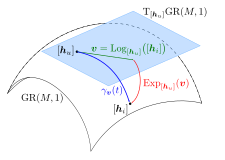
\includegraphics[width=.6\linewidth]{./figs/usch_figs/q_manifold_geodesics_h.pdf}
	\caption[Depiction of Grassmannian manifold.]{Depiction of Grassmannian manifold: we show the tangent space at $[\bm{h}_u]$, the geodesic connecting $[\bm{h}_u]$ and $[\bm{h}_i]$, the corresponding exponential and logarithm maps, and their relationships.}
	\label{usch:fig:manifold_geodesics}
\end{figure}

% Now, all ingredients are ready for unsupervised learning on the Grassmannian manifold. 


\subsection{Unsupervised CSI Clustering} \label{usch:ssec:clustering}

Among the plethora of unsupervised learning algorithms, e.g., \cite{usama19}, that are generally all useful in our user scheduling paradigm, we consider two simple and well-known data clustering methods: $K$-means clustering and agglomerative hierarchical clustering \cite{Xu15}. 
We adapt both unsupervised learning algorithms in the first step of manifold CSI clustering.
Our goal is to classify $N$ users into $K$ clusters $\{\mathcal{C}_1, \cdots, \mathcal{C}_K\}$ based on the available CSI $\{\bm{h}_u\}_{u=1}^N$ at the scheduling server such that users in each cluster exhibit high CSI similarity in the Grassmannian $\mathrm{GR}(M,1)$.


\subsubsection{Grassmannian $K$-means (GKM) Clustering } 
The basic $K$-means algorithm applies a greedy iterative approach to find a data partition that minimizes the distance between cluster members and their respective cluster centers. 
At the $t$-th iteration, the center of the $k$-th cluster $\mathcal{C}_k^t$ is defined by ${\bm{u}}_k^t \in \mathbb{C}^{M}$, which in Euclidean space is given by 
\begin{equation}\label{usch:cen}
	{{\bm{\mu}}_k^t} = \frac{1}{{\left| {{\mathcal{C}_k^t}} \right|}}\sum_{n \in {\mathcal{C}_k^t}} {{{\bm{h}}_{u}} } .
\end{equation}

In case of manifolds, the cluster centers are given by the intrinsic mean of cluster members,
\begin{align}
	\bm{\mu}_k^t=\argmin_{[\bm{u}]\in\mathrm{GR}(M,1)}\sum_{n \in {\mathcal{C}_k^t}} \dist\big([\bm{h}_u],[\bm{u}]\big),
\end{align}
which has no closed-form solution as it depends on reference points, which are not fixed. 
The computation of the intrinsic mean is shown in Algorithm~\ref{usch:alg:intrinsic_mean}, where we use the unit-vector representatives of the equivalence classes for computation.
\begin{algorithm}[htb]
	\caption{Intrinsic Mean for Cluster $k$ in $\mathrm{GR}(M,1)$}
	\label{usch:alg:intrinsic_mean}
	\begin{algorithmic}[1]
		\Statex {\textbf{Input:} $[\bm{h}_u]\in\mathcal{C}_k^t$, threshold $\epsilon$, maximum number of iterations $T_{\mathrm{im}}$}
		\State{Initialize $t=1$, $[\bm{u}]=[\bm{h}_i]$ for a random $i$ in the cluster}
		\While{$t\leq T_{\mathrm{im}}$ or $\|\bm{v}\|_{\bm{u}}\geq\epsilon$}
		\State{Compute tangent vector $\bm{v}=|\mathcal{C}_k^t|^{-1}\sum_u\mathrm{Log}_{[\bm{u}]}\big([\bm{h}_u]\big)$}
		\State{Update $[\bm{u}]=\mathrm{Exp}_{[\bm{u}]}(\bm{v})$}
		\State Set $t=t+1$
		\EndWhile
		\State Return $[\bm{\mu}_k^t]=[\bm{u}]$
	\end{algorithmic}
\end{algorithm}

For the initial centers for $K$-means clustering, namely ${\bm{\mu}}_k^0, k \in \{1,\ldots,K\}$, we can randomly select $K$ users out of the $M$ users. 
However, performance of $K$-means could suffer due to poor initialization, and instead we initialize using $K$-means++ to mitigate this effect \cite{Arthur2007kmeanspp}.

At the $t$-th iteration, each user is assigned to 
a cluster $\mathcal{C}_{k^\star}$ based on the center that is closest to the user, that is,
\begin{equation}\label{usch:assign}
	k^\star= \arg \mathop {\min }\limits_k \dist \big( [\bm{h}_u] ,[\bm{\mu}_k^t] \big).
\end{equation}
The $K$ cluster centers are updated. 
The clustering and center update steps continue until all clusters stay the same (or any other stopping criteria). 
Our implementation of Grassmannian $K$-means is summarized in Algorithm~\ref{usch:alg:grass_kmeans}.
\begin{algorithm}[htb]
	\caption{Grassmannian $K$-means}
	\label{usch:alg:grass_kmeans}
	\begin{algorithmic}[1]
		\Statex {\textbf{Input: }$\bm{h}_u\in\mathbb{C}^M,\,n\in\{1,\ldots,N\}$, intrinsic mean parameters $\epsilon$ and $T_{\mathrm{im}}$}
		\State{Normalize CSIs to obtain Grassmannian representatives.}
		\State{Set $t=0$ and $\mathcal{C}_k^0=\emptyset\,\,\forall k$}
		\State{Select initial cluster centers according to $K$-means++ using the Grassmannian distance.}
		\While{ $\mathcal{C}_k^{t}\neq\mathcal{C}_k^{t-1}$ for any $k$}
		\State Set $t=t+1$ and $\mathcal{C}_k^t=\emptyset\,\,\forall k$
		\For{each user $u$}
		\State{Find the center $[\bm{\mu}_k]$ closest to $[\bm{h}_u]$}
		\State{Assign user $u$ to $\mathcal{C}_k^t$}
		\EndFor
		\For{each cluster $k$}
		\State{Update cluster center $[\bm{\mu}_k]$ using Algorithm~\ref{usch:alg:intrinsic_mean}.}
		\EndFor
		\EndWhile
	\end{algorithmic}
\end{algorithm}

\subsubsection{Agglomerative Hierarchical Clustering (AHP)} 
This bottom-up hierarchical clustering approach begins by treating each data point as a single point cluster. 
It proceeds to successively merge the most similar cluster pairs until reaching the target number of clusters using a ``linkage'' rule to define the distances among merged pairs. 
Here, we use the complete linkage rule \cite{Xu14}, i.e., at the $t$-th agglomeration, the similarity measure between clusters ${\mathcal{C}_k^t}$ and ${\mathcal{C}_j^t}$ is 
\begin{align}
	d \left( {{\mathcal{C}_k^t},{\mathcal{C}_j^t}} \right) = \max_{\bm{h}_m\in\mathcal{C}_k^t,\,\bm{h}_u\in\mathcal{C}_j^t} \dist \big( [\bm{h}_m],[\bm{h}_u] \big) .\label{usch:eqn:complete_linkage}
\end{align}
% \begin{align}
	% 	\varphi \left( {{\mathcal{C}_k^t},{\mathcal{C}_j^t}} \right) = \frac{1}{{\left| {{\mathcal{C}_k^t}} \right|\left| {{\mathcal{C}_j^t}} \right|}}\sum\limits_{m \in {\mathcal{C}_k^t}} {\sum\limits_{n \in {\mathcal{C}_j^t}} {\beta \left( {{{\bm{h}}_{m}},{{\bm{h}}_{u}} } \right)} } .\label{usch:eqn:avg_linkage}
	% \end{align}

In particular, the linkage between two single-user clusters is $d \left( \mathcal{C}_m^t,\mathcal{C}_u^t \right) =\dist \big( [\bm{h}_m],[\bm{h}_u] \big)$. Given a set of clusters $\{\mathcal{C}_1^t,\cdots, \mathcal{C}_{K'}^t\}$, where $K'\geq K$, at each iteration, we determine the most similar pairs of clusters according to the linkage rule (\ref{usch:eqn:complete_linkage}). 
After merging the two closest clusters, the process is repeated on the new set of clusters until the target number of clusters $K$ is reached.

Note that in the context of Grassmannian manifold framework, any
effective clustering approach is a valid option. 
We only focus on the two simpler approaches for their low complexity and ease of exposition. 
% Other probabilistic extensions of clustering algorithms, e.g., Expectation-Maximization 
% algorithm \cite{em}, can also be applied.






\subsection{CSI-Based User Scheduling} \label{usch:ssec:grouping}

\subsubsection{Direct Greedy Scheduling}
One way to control CCI among users scheduled in the same group is to apply a simple greedy algorithm to form RSGs. 
This direct greedy method can be used a basic benchmark. 
Starting from a user group of one random user, we can consider each new user by examining its pairwise CSI correlation with all users in the group against a set threshold $\beta$, and only add the new user if each pairwise correlation is below $\beta$ until the group size reaches $M$.  We can then continue to schedule additional groups. 
This \textbf{direct greedy scheduling}, which we denote DS, does not rely on any supervised learning. 
Its scheduling results would vary significantly according to the order of the users being considered during scheduling. 


\subsubsection{User Scheduling with Unsupervised Learning}
MIMO user scheduling optimization can consider different performance criteria.
However, co-channel interference (CCI) among users scheduled for the same RSG should always reduced for any sensible performance metric. 
Based on the outcomes of CSI clustering, users within the same cluster have highly similar CSIs in terms of strong pairwise correlation coefficient, which can lead to strong CCI and challenge the receiving accuracy. 
From this perspective, users from different clusters are dissimilar and should induce low CCI, and thus are good candidates to be scheduled for MIMO resource sharing.

Our proposed GKM and AHP algorithms exploit the outcomes from CSI learning in the form of CSI clusters.  
Since there are multiple CSI clusters, our proposed GKM scheduling would compute the inter-cluster distances and sort clusters in descending order of minimum inter-cluster distance. 
We can then start GKM scheduling by forming user scheduling groups by considering clusters that are as far apart as possible to contain CCI.  
In the case of AHP, we apply cluster merging from the smallest cluster sizes.


\subsection{Power Control in MAC Scheduling} 

CSI gains and power control must be considered differently in MAC and BC scheduling systems.
In MAC, different receiver designs will benefit from different strategies: 
joint MMSE receiver benefits from CSIs with similar gains, whereas interference cancellation (e.g. SIC) receiver thrives when CSIs have
large gain differences. 
In practice, power control in MAC plays an important role to mitigate the near-far problem. 
It is well known that optimal power control is achieved by waterfilling with respect to a target interference and noise level \cite{Tse05}.
However, it can be hard to accurately apply power control at the scheduling stage for a large number of distinct groups. 
Thus, we can consider two scenarios: (a) equal power transmission, where maximum user transmit power $p_u=p_{\mathrm{UE}}^{\mathrm{max}}$ is used for all $u$ without power control, despite having different channel gains $\|\bm{h}_u\|$ (MAC-U); (b) effective power control such that $p_u\|\bm{h}_u\|^2$ is nearly constant at the receiver (MAC-P). 

Consider each user signal quality in MAC. 
Note that using an MMSE receiver with $\sigma^2$ being the noise power, the resulting user SINR is 
\begin{align*}
	\SINR_u^{\MAC} =
	\frac{\bm{h}_u\herm}{\|\bm{h}_u\|^2}\Bigg(\frac{\sigma^2\bm{I}}{p_u\|\bm{h}_u\|^2}+\sum_{i\in\mathcal{S}_g,i\neq n}\frac{p_i\bm{h}_i\bm{h}_i\herm}{p_u\|\bm{h}_u\|^2}\Bigg)^{-1}\bm{h}_u,
\end{align*}
which means that SINR depends on all pairwise correlations of users within a group and the ratio of their received powers. 
Hence, the MMSE receiver benefits when the users within a group have similar received power $p_u\|\bm{h}_u\|^2$, and thus the received power ratios are close to 1. 
Such power ratios have minimum near-far effect and more consistent performance. 
These power ratios are often achieved under power control. 
% We assume that $p^{\mathrm{max}}$ is large enough that it can compensate small CSI gains.
Hence, we define the following grouping rule for MAC-P:
\begin{align}
	\varphi _{\mathrm{P}}
	^{\MAC}(\bm{h}_u,\mathcal{S}_g)=\left\{\begin{array}{ll}1&
		\rho(\bm{h}_u,\bm{h}_{\ell})\leq\beta\,\,\,\forall \ell\in\mathcal{S}_g
		\,\,\wedge\,\,\, |\mathcal{S}_g|<M,
		\\0&\text{otherwise.}\end{array}\right.
	\label{usch:eqn:assignment_rule_macp}
\end{align}
% \begin{align}
	%     \varphi _{\mathrm{P}}
	%     ^{\MAC}(\bm{h}_u,\mathcal{S}_g)=\left\{\begin{array}{ll}1&
		%     \begin{array}{l}\rho(\bm{h}_u,\bm{h}_{\ell})\leq\beta\,\,\,\forall \ell\in\mathcal{S}_g\\
			%     \,\,\wedge\,\,\, |\mathcal{S}_g|<M\end{array},\\0&\text{otherwise.}\end{array}\right.
	%     \label{usch:eqn:assignment_rule_macp}
	% \end{align}

\subsection{MAC Scheduling without Power Control} 

In large scale systems such as IoT deployment, power control may not be practical. 
Without power control (MAC-U), our proposed scheduling algorithm
shall attempt to reduce CCI by forming RSGs of similar channel gain 
and low similarity. 

Specifically, we partition CSI gains of all $N$ users into $B$ levels.
Users scheduled in group $\mathcal{S}_g$ must have CSI belonging to the same partition.
Hence, we modify the grouping rule $\varphi_{\mathrm{P}}^{\MAC}$ to include this additional criteria: 
\begin{align}
	\varphi_{\mathrm{U}}^{\MAC}(\bm{h}_u,\mathcal{S}_g)=\left\{\begin{array}{ll}1&
		\rho(\bm{h}_u,\bm{h}_{\ell})\leq\beta\,\,\,\forall \ell\in\mathcal{S}_g
		\,\,\wedge\,\,\, |\mathcal{S}_g|<M
		\,\,\wedge\,\,\|\bm{h}_u\|\in b(\mathcal{S}_g),\\0&\text{otherwise.}\end{array}\right.
	\label{usch:eqn:assignment_rule_mac}
\end{align}
% \begin{align}
	%     \varphi_{\mathrm{U}}^{\MAC}(\bm{h}_u,\mathcal{S}_g)=\left\{\begin{array}{ll}1&
		%     \begin{array}{l}\rho(\bm{h}_u,\bm{h}_{\ell})\leq\beta\,\,\,\forall \ell\in\mathcal{S}_g\\
			%     \,\,\wedge\,\,\, |\mathcal{S}_g|<M\\
			%     \,\,\wedge\,\,\|\bm{h}_u\|\in b(\mathcal{S}_g)\end{array},\\0&\text{otherwise.}\end{array}\right.
	%     \label{usch:eqn:assignment_rule_mac}
	% \end{align}

\subsection{BC Scheduling for Low Complexity Transceivers} 

Practical individual receivers in BC systems do not share CSI information.
For massive deployment, dirty paper coding (DPC) \cite{jindal2005dirty} is also challenging to
implement practically.  Our user scheduling will target low complexity
transceivers that only utilize local CSI. Therefore, power control for scheduled user
groups could prove useful. We consider a simple power control by allocating
uniform transmit power among BC group members, i.e. $p_u=p_{\mathrm{BS}}^{\mathrm{max}}|\mathcal{S}_g|^{-1}$. 
Other simple schemes could be applied, e.g. allocating power such that users within a group exhibit close to identical received signal power $p_u\|\bm{h}_i\|^2$.
% , i.e., we set $p_u=p_{\mathrm{BS}}^{\mathrm{max}}(\|\bm{h}_u\|^2|\mathcal{S}_g|)^{-1}$.


Furthermore, users with weaker CSI gain experience lower SNR. To compensate, our BC scheduling algorithm considers the CSI gain and allocate fewer users of similarly low
CSI gain into an RSG to maintain sufficiently high SINR. 
As a simple two-tier implementation example, 
we shall partition downlink CSI gains into two levels with a threshold $\delta$.
We assign users with weaker CSI gains below $\delta$ into weaker CSI groups,
up to a maximum of $E$ users in such groups. Conversely, we assign users with stronger CSI gains above $\delta$ into stronger CSI groups, up to a maximum of $D$ users in such groups where $D\ge E.$

The corresponding grouping rule is:
% \begin{align}
	%     \varphi^{\BC}(\bm{h}_u,\mathcal{S}_g)=\left\{\begin{array}{ll}1&\rho(\bm{h}_u,\bm{h}_{\ell})<\beta\,\,\,\forall \ell\in\mathcal{S}_g,\\
		%     &\,\,\wedge\,\,\, |\mathcal{S}_g|<M\\0&\text{otherwise.}\end{array}\right.
	% \end{align}
\begin{align}
	\varphi^{\BC}(\bm{h}_u,\mathcal{S}_g)=\left\{\begin{array}{ll}1&
		\rho(\bm{h}_u,\bm{h}_{\ell})\leq\beta
		\,\,\wedge\,\,|\mathcal{S}_g|<E\,\,\wedge\,\,\|\bm{h}_u\|,\|\bm{h}_{\ell}\|\leq\delta,\,\,\,\,\forall \ell\in\mathcal{S}_g,\\
		1&
		\rho(\bm{h}_u,\bm{h}_{\ell})\leq\beta
		\,\,\wedge\,\,|\mathcal{S}_g|<D\,\,\wedge\,\,\|\bm{h}_u\|,\|\bm{h}_{\ell}\|>\delta,\,\,\,\,\forall \ell\in\mathcal{S}_g\\
		0&\text{otherwise.}\end{array}\right.
	\label{usch:eqn:assignment_rule_bc}
\end{align}

To summarize, Figure~\ref{usch:fig:similarity_assisted_scheduling} depicts a flowchart of a greedy algorithm under our proposed user scheduling principle based on unsupervised learning outcomes. 
The application for uplink MAC-P, MAC-U or downlink BC depends on the choice of the 
selection rule $\varphi(\bm{h}_u,\mathcal{S}_g)$ 
according to (\ref{usch:eqn:assignment_rule_macp}), (\ref{usch:eqn:assignment_rule_mac}) or (\ref{usch:eqn:assignment_rule_bc}), respectively. Moreover, DS uses the same grouping rules for benchmarking purposes.
\begin{figure}[tbp]
\centering
\includegraphics[width=.56\linewidth]{./figs/usch_figs/ClusterAssitedSchedulingAlgorithm.pdf}
\caption[Flowchart of a greedy algorithm under the proposed scheduling principle.]{Flowchart of a greedy algorithm under the proposed scheduling principle, using rule (\ref{usch:eqn:assignment_rule_macp}) for MAC-P, (\ref{usch:eqn:assignment_rule_mac}) for MAC-U and (\ref{usch:eqn:assignment_rule_bc}) for BC.}
\label{usch:fig:similarity_assisted_scheduling}
\end{figure}

More generally, variants of the proposed scheduling algorithm can exploit both the knowledge of CSI similarity and CSI gains in different ways without changing significantly the underlying methodology supporting our proposed strategy. 
Even more broadly, the unsupervised learning paradigm can also accommodate CSI features based on system performance and design choices. 

\subsection{Complexity Analysis}
\subsubsection{Clustering}
First, we determine the complexity of Grassmannian $K$-means as follows:
\begin{itemize}
\item The CSI normalization step has a cost of $\mathcal{O}(MN)$.
\item The Grassmannian distance has a cost of $\mathcal{O}(M)$, and thus the $k$-means++ initialization has a cost of $\mathcal{O}(KMN)$.
\item Each iteration of the algorithm consists on two steps. First, assigning $N$ users to $K$ clusters, with a total cost of $\mathcal{O}(KMN)$. Then, the cluster center update for $K$ clusters, which requires the computation of $N$ logarithm maps and $K$ exponential maps, both operations with a cost of $\mathcal{O}(M)$. This process is iterative, but in practice takes only a few intrinsic mean iterations and the cost of center updates is $\mathcal{O}(KMN)$.
\end{itemize}
Accordingly, the total cost for $t$ iterations of  Grassmannian $K$-means is $\mathcal{O}(tKMN)$.

In the case of Agglomerative Hierarchical Clustering, optimal implementations depend on the linkage criteria \cite{zaki14}.
When considering complete linkage, it is known that the optimal algorithm has complexity $\mathcal{O}(N^2)$ with respect to similarity comparisons. 
Furthermore, the pairwise CSI correlation has a total cost of $\mathcal{O}(MN^2)$ as there are $N(N-1)$ pairwise computations, and thus the complexity of this clustering approach is $\mathcal{O}(MN^2)$.

\subsubsection{User Grouping}
All user grouping approaches (similarity-assisted and DS) exploit pairwise correlation information, which has cost $\mathcal{O}(M)$.
For the similarity-assisted approaches (GKM and AHP), the algorithm checks $K-1$ clusters with a total of $N'=N-|\mathcal{C}_k^*|$ users, which we can approximate in average with an uniform partition as $N'=N-N/K=N(K-1)/K$. In the case of DS, there is no clustering information, and hence $N-1$ users need to be tested for assignment.
Hence, the computation complexity of similarity-assisted methods and DS is of order $\mathcal{O}(MN)$. Of course, in average we expect to observe some computational gains in similarity-assisted grouping, depending on system parameters and selected threshold, but cannot guarantee that they are going to be dramatically significant.

\section{Numerical Experiments}\label{usch:sec:sim}
In this section we test our proposed scheduling principle based on unsupervised learning. 
Considering a variety of user service needs and CSI properties, we provide a simple MIMO system model for both uplink and downlink applications. 


We examined one BS equipped with $M=8$ antennas, serving $N$ single-antenna users. 
The mobile user CSI in uplink/downlink is modeled as random vectors that incorporate both shadowing
and Rayleigh fading. 
A circularly complex normal vector of size $M$ represents MIMO Rayleigh fading.
The shadowing effect is modeled as a power gain that follows a lognormal distribution, with zero mean and standard deviation $\sigma_L$ of 3dB in logarithmic scale. 
Additive channel noise is included in both uplink/downlink directions, corresponding to 20dB of average SNR. 

We generate 100 different channels and perform 10 runs per channel realization in our Monte-Carlo simulations. 
All tests are performed in MATLAB using a 64-bit Windows PC  with an i7-7700K processor and 32GB RAM.

\subsection{Performance Metrics}
\subsubsection{Clustering}
Though our scheduling method is compatible with any clustering algorithm, we adopt the well known and simple $K$-means clustering algorithms, though other clustering algorithms would have been equally applicable.

Recall that $K$-means clustering begins a pre-determined cluster number $K$. 
However, choosing the best $K$ is a non-trivial problem which is problem dependent and does not have a best consensus solution \cite{gap}.
Still there are several metrics that can help determine the number of clusters, such as the Silhouette value \cite{silhouette}, the Krzanowski-Lai index \cite{Lai}, and the Hartigan index \cite{Hartigan}. 
Regardless, we know that the nature of the MAC and BC systems imply that RSGs cannot have more than $M$ users, since more users necessarily lead to more ill-conditioned group CSI matrix, impacting performance significantly. Hence, we set the number of clusters to be $K\leq M$ depending on the scenario, and show the pairwise correlation matrices obtained with both clustering methods. 


\subsubsection{CCI Evaluation}
CCI leads a loss of signal-to-interference and noise ratio (SINR) in reference to SNR. 
To evaluate the efficacy of user scheduling, we compute the loss in SINR that each user experiences. 
In other words, we normalize the SINR of user $u$ by its SNR if it were scheduled without co-channel users (a singleton group), such that it does not share resources and is only hampered by noise. 
Let $p_u$ be the transmit power of the $u$-th user and $\sigma^2$ be the additive channel noise variance. 
This SINR loss is given by
\begin{align}
10 \log_{10}\bigg(	\frac{\SINR_u}{p_u\|\bm{h}_u\|^2/\sigma^2}\bigg) \; \mbox{dB}.\label{usch:eqn:normalized_sinr}
\end{align}
Thus, 0dB SINR loss corresponds fully orthogonal CSIs among co-channel users and zero CCI. 
 
 
\subsubsection{Resource Efficiency}
To compare how well each scheduling method utilizes limited spectrum resources, we consider the overall MIMO spectrum efficiency by assuming that each scheduled MIMO user group is allocated the same bandwidth (or same
amount of spectrum resource). 
In such case, the spectrum efficiency of the scheduling can be measured by 
averaging the  achieved sum-rate of all groups over $G$ total RSGs: 
$
\frac{1}{G}\sum_{g=1}^G R_{g}.
$


\subsubsection{Runtime}
As a proxy for computational complexity, in all simulations we store the ``wall-clock'' time for successful execution of the algorithms under test. 
Naturally, runtime often depends on computer, platform and code implementation. 
Thus, runtime by itself it may not fully capture the complexity of scheduling algorithms. 
Hence, we apply the same built-in functions, establish similar program structure and implementation for all algorithms under test to mitigate platform biases.
Additionally, we also test scheduling for different number of users $N$ to compare the scalability of the algorithms. 

\subsection{Uplink MAC MIMO Performance}
In MAC, we set the number of clusters to $K=8$ and we adopt linear MMSE receiver based on CSI of all received user signals in an RSG.  
This choice of $K$ ensures that the scheduling process will attempt to utilize all spatial degrees of freedom for high spectrum efficiency. 

\subsubsection{Clustering Outcomes}
\begin{figure}[ht]
\centering
\begin{subfigure}[b]{0.48\linewidth}
	% Caption before figure
	\centering
	\includegraphics[width=.95\linewidth]{./figs/usch_figs/pairwise_corr_all_users_GKM_M8_N800_K8.pdf}
	\subcaption{GKM.}\label{usch:fig:pwc_gkm_mac}
\end{subfigure}
% 	\hfill
\begin{subfigure}[b]{0.48\linewidth}
	% Caption before figure
	\centering
	\includegraphics[width=.95\linewidth]{./figs/usch_figs/pairwise_corr_all_users_AHP_M8_N800_K8.pdf}
	\subcaption{AHP.} \label{usch:fig:pwc_AHP_mac}
\end{subfigure}
\caption[Example of pairwise CSI correlation coefficient matrices after clustering $N=800$ users with $K=8$ clusters.]{Example of pairwise CSI correlation coefficient matrices after clustering $N=800$ users with $K=8$ clusters. Larger correlation values are darker. 
	(\subref{usch:fig:pwc_gkm_mac}) Grassmannian $K$-means. (\subref{usch:fig:pwc_AHP_mac}) Hierarchical Clustering.}
\label{usch:fig:clusters_pwc_M8_N800}
\end{figure}
Figure~\ref{usch:fig:clusters_pwc_M8_N800} shows the pairwise correlation matrix of $N=800$ user CSIs after GKM and AHP clustering. 
Using grayscale of $[0,1]$, larger values correspond to darker colors. 
An ideal clustering outcome should show 8 blocks of darker squares along the diagonal. 
GKM yields user clusters that show strong within-cluster similarity to be used later in scheduling. 
All 8 clusters contain many pairs that exhibit high spatial correlation. 
AHP shows less defined clusters: each cluster exhibits less highly correlated pairs, or in other words, users have weaker CSI correlation (i.e. weaker similarity) within each cluster. 


\subsubsection{Scheduling Performance}


To systematically evaluate the the effect of exploiting similarity identified during clustering, we analyze our approach in MAC by considering the two scenarios described in the previous section:
\begin{enumerate}
\item perfect power control, where each received user signal has  
unit power, i.e. $p_u\|\bm{h}_u\|^2=1\,\forall n\in\{1,\ldots,N\}$, denoted as MAC-P;
\item no power control, where user CSI powers follow a log-normal distribution with parameter 3 dB, and $p_u=p_{\mathrm{UE}}^{\mathrm{max}}=1$ for all $u$, denoted as MAC-U.
\end{enumerate}

\begin{figure*}[ht]
\centering
\begin{subfigure}{0.48\linewidth}
	\centering
	\includegraphics[width=.95\linewidth]{./figs/usch_figs/MACU_AvgUserSINRLoss_normalizedChannelPwr_noPwrCtrl_M8_N800_nSim10_nChannel100_K08_sigman2_-20.pdf}
	\caption{Average user SINR loss.}\label{usch:fig:MACU_sinrLoss_M8_N800}
\end{subfigure}
\begin{subfigure}{0.48\linewidth}
	\centering
	\includegraphics[width=.95\linewidth]{./figs/usch_figs/MACU_NormalizedEfficiency_normalizedChannelPwr_noPwrCtrl_M8_N800_nSim10_nChannel100_K08_sigman2_-20.pdf}
	\caption{Average efficiency. }
	\label{usch:fig:MACU_efficiency_M8_N800}
\end{subfigure}
\caption[Performance of all scheduling algorithms in MAC with perfect power control (MAC-P).]{Performance of all scheduling algorithms in MAC with perfect power control (MAC-P). Here, $M=K=8$ and $N=800$. Solid lines represent the average over channel realizations, and shaded areas show all values within the 10th and 90th percentiles.}
\label{usch:fig:MACU_M8_N800}
\end{figure*}
\begin{figure*}[ht]
\centering
\begin{subfigure}{0.48\linewidth}
	\centering
	\includegraphics[width=.95\linewidth]{./figs/usch_figs/MACP_AvgUserSINRLoss_normalizedChannelPwr_PwrCtrl_M8_N800_nSim10_nChannel100_K08_sigman2_-20.pdf}
	\caption{Average user SINR loss.}\label{usch:fig:MACP_sinrLoss_M8_N800}
\end{subfigure}
\begin{subfigure}{0.48\linewidth}
	\centering
	\includegraphics[width=.95\linewidth]{./figs/usch_figs/MACP_NormalizedEfficiency_normalizedChannelPwr_PwrCtrl_M8_N800_nSim10_nChannel100_K08_sigman2_-20.pdf}
	\caption{Average efficiency. }
	\label{usch:fig:MACP_efficiency_M8_N800}
\end{subfigure}
\caption[Performance of all scheduling algorithms in MAC without power control (MAC-U).]{Performance of all scheduling algorithms in MAC without power control (MAC-U). Here, $M=K=8$ and $N=800$. Solid lines represent the average over channel realizations, and shaded areas show all values within the 10th and 90th percentiles.}
\label{usch:fig:MACP_M8_N800}
\end{figure*} 

We first test the MAC-P scenario, which helps isolate the benefits of unsupervised learning without the effect of variable receive powers. We consider three scheduling algorithms: the proposed GKM scheduling, AHP scheduling, and DS scheduling. 
For these three methods, Figure~\ref{usch:fig:MACU_sinrLoss_M8_N800} shows the comparison of SINR mean and SINR distribution (10\% to 90\% percentiles) of the resulting user SINR loss. The corresponding spectral efficiency is shown in Figure~\ref{usch:fig:MACU_efficiency_M8_N800}.

From our test results, when $\beta$ is set low, only very small amount of CCI is tolerated. 
In such cases, scheduling performance continues to be dominated by channel noise (i.e., SNR) and allowing little if any resource-sharing. 
Thus it is natural that, for $\beta <0.25$, all three scheduling algorithms exhibit little SINR loss and relatively low spectrum efficiency. 
As we increase $\beta$, the spectrum efficiency starts go grow for all algorithms, as shown in Figure~\ref{usch:fig:MACU_efficiency_M8_N800}. 
Eventually, spectrum efficiency of both GKM and AHP saturate.  
More specifically, GKM achieves higher spectrum efficiency but also larger SINR loss. 
AHP on the other hand, achieves lower spectrum efficiency but also lower SINR loss. 
In terms of SINR loss, both GKM and AHP exhibit very modest amount of SINR loss that saturates at 2dB and 1dB on average, respectively. 
These tests show that MIMO user scheduling can achieve spectrum efficiency and SINR loss tradeoff, with GKM being more efficient in spectrum utilization. 

For DS, spectrum efficiency would peak at $\beta=0.35$ before decreasing with increasing $\beta$. 
The spread of SINR is also large for DS, with some users experimenting more than -12dB of SINR loss. 
Both GKM and AHP have a tighter spread, which means most of the users will only experience 5dB of loss at most for GKM, and 2dB for AHP. 
This demonstrates the failure of DS in grouping users of low mutual CCI to achieve good tradeoff between spectrum efficiency and SINR loss.

We next test the more practical case of unequal CSI gains in
a network without power control, MAC-U. Against users of unequal CSI gain, for the scheduling rule $\varphi_{\mathrm{U}}^{\MAC}$ we partition users according to their CSI powers uniformly with power interval of $3$ dB such that users are divided according to power level boundaries of $\ldots,-4.5,-1.5,1.5,4.5,\ldots$ in dB. 
Figs.\ref{usch:fig:MACP_sinrLoss_M8_N800} and~\ref{usch:fig:MACP_efficiency_M8_N800} show the SINR loss and average efficiency of all methods in MAC-U.

Again we observe that for smaller $\beta$, channel noise dominates the scheduling performance and all algorithms attain similar performance. With increasing $\beta$, users experience more SINR losses as more of them share resources, while the system enjoys the corresponding improvement in spectrum efficiency. The efficiency of GKM and AHP saturate for large $\beta$, with a modest increase of 1dB of SINR loss in average compared to MAC-U. Again, GKM achieves better performance with a small tradeoff in user SINR, compared to AHP that grants better user SINR at the expense of reduced efficiency. These tests confirm that similarity-assisted methods improve MIMO user scheduling, even when considering random channel gains and uniform power allocation.

In contrast, DS achieves peak efficiency at $\beta=0.35$ and decreases steadily for larger $\beta$. 
It also incurs greater SINR losses without any benefit in spectrum efficiency, being smaller than the efficiency of GKM and AHP in almost all cases. 
In average, users experience 7dB of SINR loss, and even more, the users that experience the largest losses are at least 4dB worse than with GKM or AHP. 
It is clear that DS offers no reasonable tradeoff between user SINR and spectral efficiency.

Additionally, note that the performance of MAC-P is naturally better than MAC-U, as the former enjoys perfect power control and can effectively deal with CSI power variability. Nevertheless, our proposed algorithms still attain good performance under the simpler setup of MAC-U, with only minor performance loss.

In both MAC-U and MAC-P tests, GKM and AHP scheduling deliver much better spectrum efficiency and lower SINR loss.
Compared with DS, our tests strongly support the efficacy of the proposed MIMO user scheduling principle based on unsupervised learning on the Grassmannian manifold. 


\subsection{Performance for Downlink (BC)}
In BC, we set the number of clusters to $K=4$. Recall that the MRT precoders do not exploit the CSI of users in an RSG, and hence a smaller $K$ better controls the SINR experienced by each user without incurring in severe degradation, due to oversharing resources. 
\subsubsection{Clustering Outcomes}
We first analyze the CSI correlation matrices for GKM and AHP in Figure~\ref{usch:fig:clusters_pwc_M8_K4_N800}, where darker colors in
grayscale denote larger correlation coefficient. Even for a low number of clusters, GKM is able to produce discriminative clusters that contain several user pairs with relatively high correlation compared to the members of other clusters. In this case, however, AHP produces clusters with fairly lower correlation, hinting that users within a cluster are not highly similar. This can also be explained by the bottom-up nature of hierarchical clustering of large datasets, as the last steps (merging large subclusters) are not very discriminative.
\begin{figure}[htb]
	\centering
	\begin{subfigure}[b]{0.48\linewidth}
		% Caption before figure
		\centering
		\includegraphics[width=.95\linewidth]{./figs/usch_figs/pairwise_corr_all_users_GKM_M8_N800_K4.pdf}
		\subcaption{GKM.}\label{usch:fig:pwc_gkm_bc}
	\end{subfigure}
	\begin{subfigure}[b]{0.48\linewidth}
		% Caption before figure
		\centering
		\includegraphics[width=.95\linewidth]{./figs/usch_figs/pairwise_corr_all_users_AHP_M8_N800_K4.pdf}
		\subcaption{AHP.} \label{usch:fig:pwc_AHP_bc}
	\end{subfigure}\hfill
	\caption[Example of pairwise CSI correlation coefficient matrices after clustering $N=800$ users with $K=4$ clusters.]{Example of pairwise CSI correlation coefficient matrices after clustering $N=800$ users with $K=4$ clusters. Larger correlation values are darker. 
		(\subref{usch:fig:pwc_gkm_bc}) Grassmannian $K$-means. (\subref{usch:fig:pwc_AHP_bc}) Hierarchical Clustering.}
	\label{usch:fig:clusters_pwc_M8_K4_N800}
\end{figure}

\subsubsection{Scheduling Performance}
For BC systems, we only consider the case where all users have random log-normal distributed CSI power, as the SINR of each user does not depend on the power of the rest of the co-channel users.
Here, for the BC grouping rule $\varphi^{\BC}$ we consider a maximum number of users $D=K=4$, a gain threshold for weak users $\delta=0.5$ corresponding to -6dB of CSI power with respect to the average channel power, and a maximum number of weak users in an exclusive group $E=2$. We also set $p_{\mathrm{BS}}^{\mathrm{max}}=M$ and use uniform power allocation within scheduled groups, although a different scheme can also apply.

Figs.~\ref{usch:fig:MACP_sinrLoss_M8_N800} and~\ref{usch:fig:MACP_efficiency_M8_N800} depict the SINR loss distribution and corresponding spectrum efficiency of all tested scheduling methods in BC. 
We first observe higher achieved SINR loss for BC than for MAC.
Such outcome is expected since the selected UE receiver cannot utilize CSI of other users in its co-channel MIMO group. 
Correspondingly, the BC spectrum efficiency is lower.
Similar to MAC systems, all three methods under comparison show comparable performance in terms of efficiency and SINR loss for $\beta\leq0.15$. 
For larger $\beta$, AHP stalls and GKM offers a modest growth in efficiency, reaching 13\% higher efficiency than AHP for $\beta>0.3$. 
By comparison, AHP scheduling shows the best SINR losses, whereas GKM offers a good tradeoff and outperforms AHP in spectral efficiency over all values of $\beta$.

In BC, the efficiency of DS peaks at at $\beta=0.2$ before dropping by 58\% from its peak.
Both the proposed GKM and AHP out-perform DS for $\beta\geq 0.25$. 
DS also suffers the worst losses for all users, with an average SINR loss of up to 12dB, and 18dB SINR loss for the 10\% of users that experience the worst conditions. Moreover, most users experience significantly worse SINR conditions on DS than GKM or AHP. 
Clearly, our test results in BC show that our proposed scheduling strategy, by exploiting similarity obtained via unsupervised learning, provides better SINR for the UE receivers and achieve higher spectrum efficiency than a direct approach.
\begin{figure*}[ht]
	\centering
	\begin{subfigure}{0.48\linewidth}
		\centering
		\includegraphics[width=.95\linewidth]{./figs/usch_figs/BCP_AvgUserSINRLoss_normalizedChannelPwr_M8_N800_nSim10_nChannel100_K04_sigman2_-20.pdf}
		\caption{Average user SINR loss.}\label{usch:fig:BCP_sinrLoss_M8_N800}
	\end{subfigure}
	\begin{subfigure}{0.48\linewidth}
		\centering
		\includegraphics[width=.95\linewidth]{./figs/usch_figs/BCP_NormalizedEfficiency_normalizedChannelPwr_M8_N800_nSim10_nChannel100_K04_sigman2_-20.pdf}
		\caption{Average efficiency. }
		\label{usch:fig:BCP_efficiency_M8_N800}
	\end{subfigure}
	\caption[Performance of all scheduling algorithms in BC.]{Performance of all scheduling algorithms in BC. Here, $M=8$, $N=800$, $K=D=4$, $E=2$ and $\delta=0.5$. Solid lines represent the average over channel realizations, and shaded areas show all values within the 10th and 90th percentiles.}
	\label{usch:fig:BCP_M8_N800}
\end{figure*}

\subsection{Runtime and Scalability}
Table~\ref{usch:tab:runtime} summarizes the average runtime of all 3 algorithms under test for various number of users $N$ under the same test settings specified earlier. 
In particular, we set a correlation threshold of $\beta=0.8$, where there is significant performance difference between DS and the two proposed methods based on learning. 
As expected, the runtime grows with increasing $N$ in both uplink and downlink. 
The runtime is not affected by different channel gains (MAC-P vs. MAC-U). 
Because of its clustering complexity, AHP requires the largest runtime, whereas DS can be faster without clustering for smaller number of users. 
On the other hand, the proposed GKM only requires a modest level of computation, in view of the performance benefits shown in terms of SINR loss and spectrum efficiency. 
For
example, GKM scheduling under uplink MAC only requires 
a modest increase of computation to provide significant performance improvement with respect to DS. 
For larger number of nodes $N$, the runtime of GKM scheduling scales mildly, as opposed to the sharper rise of runtime for AHP. 
In BC downlink, we observe similar results, in which the complexity gap between GKM scheduling and DS is less significant. 
The BC runtime comparison shows that for large $N$ deployment smart scheduling methods based on unsupervised learning offer improved performance with little or no increase in computation complexity. 

\begin{table}[htb]
\centering    
\caption{Average runtime of all algorithms, in seconds, for $\beta=0.8$.}
\label{usch:tab:runtime}
% \renewcommand{\arraystretch}{1.1}
\begin{tabular}{cc||ccc|ccc||ccc}
	& Mode & \multicolumn{3}{c|}{MAC-P} & \multicolumn{3}{c||}{MAC-U} & \multicolumn{3}{c}{BC}\\
	& Method & GKM & AHP & DS & GKM & AHP & DS  & GKM & AHP & DS \\\hline
	\multirow{5}{*}{$N$}
	& $800$  & 0.41 & 0.77 & 0.11 & 0.42& 0.78& 0.11 & 0.76& 1.22& 0.38\\
	& $1600$ & 1.97& 4.05& 0.96&2.03&4.12& 1.00& 2.96& 6.29& 3.03\\
	& $2400$ & 5.95&11.02&2.85&6.05&10.99&2.87&8.41&13.78&8.93\\
	& $3200$ &11.20&25.28&8.37&11.47&25.69&8.08&19.30&32.45&22.93 \\
	& $4000$ & 20.25&42.56&14.29&20.29&41.98&14.27&36.21&54.12&40.74\\
\end{tabular}
\end{table}

% \begin{tabular}{ccccccc}
%     & & \multicolumn{5}{c}{$N$}\\\cline{3-7}
%      Mode & Method & $800$ & $1600$ & $2400$ & $3200$ & $4000$ \\\hline\hline
%      \multirow{3}{*}{MAC-P}
%      & GKM    & 0.41 & 1.97 &  5.95 & 11.20 & 20.25 \\ \cline{2-7}
%      & AHP    & 0.77 & 4.05 & 11.02 & 25.28 & 42.56 \\ \cline{2-7}
%      & DS & 0.11 & 0.96 &  2.85 &  8.37 & 14.29 \\ \hline
%      \multirow{3}{*}{MAC-U}
%      & GKM    & 0.42 & 2.03 &  6.05 & 11.47 & 20.29 \\ \cline{2-7}
%      & AHP    & 0.78 & 4.12 & 10.99 & 25.63 & 41.98 \\ \cline{2-7}
%      & DS & 0.11 & 1.00 &  2.87 &  8.08 & 14.27 \\ \hline\hline\multirow{3}{*}{BC}
%      & GKM    & 0.76 & 2.96 &  8.41 & 19.30 & 36.21 \\ \cline{2-7}
%      & AHP    & 1.22 & 6.29 & 13.78 & 32.45 & 54.12 \\ \cline{2-7}
%      & DS & 0.38 & 3.03 &  8.93 & 22.93 & 40.74 \\ \hline 
% \end{tabular}

\section{Summary}
In this chapter, we investigated the NP-hard problem of MIMO user scheduling in a general setting for large scale networks. We considered both uplink (MAC) and downlink (BC) operation. Recognizing the computational complexity of  of traditional solutions due to network size, and the difficulties inherent to direct application of machine learning schemes, we proposed a new two-step paradigm for scalable MIMO user scheduling. 
In the first step, our method implemented unsupervised learning to identify users with highly similar CSI. This goal is achieved by clustering CSIs in the complex Grassmannian manifold, where distances are directly related to spatial diversity. In the second step, a simple greedy scheduling scheme exploited the learned similarities to schedule user groups with high CSI diversity, minimizing co-channel interference. Our numerical tests demonstrated substantial performance gains and robustness of similarity-assisted scheduling when compared to direct scheduling, both in terms of user SINR and spectrum efficiency, with a modest increase in computational effort.